% DO NOT COMPILE THIS FILE DIRECTLY!
% This is included by the other .tex files.

\lstdefinelanguage{json}{
    basicstyle=\ttfamily\footnotesize,
    numbers=left,
    numberstyle=\ttfamily\footnotesize,
    stepnumber=1,
    numbersep=8pt,
    showstringspaces=false,
    breaklines=true,
    frame=lines,
    title=\lstname,
    backgroundcolor=\color{background},
    literate=
     *{0}{{{\color{numb}0}}}{1}
      {1}{{{\color{numb}1}}}{1}
      {2}{{{\color{numb}2}}}{1}
      {3}{{{\color{numb}3}}}{1}
      {4}{{{\color{numb}4}}}{1}
      {5}{{{\color{numb}5}}}{1}
      {6}{{{\color{numb}6}}}{1}
      {7}{{{\color{numb}7}}}{1}
      {8}{{{\color{numb}8}}}{1}
      {9}{{{\color{numb}9}}}{1},
}


\begin{frame}
\titlepage
\end{frame}

\begin{frame}
  \frametitle{Dashboard in MISP}
  \begin{itemize}
    \item User configurable simple dashboard interface
    \item {\bf Visualise}, {\bf aggregate} and {\bf track} data important to you
    \item Brand new feature, still undergoing reworks
  \end{itemize}
  \begin{center}
    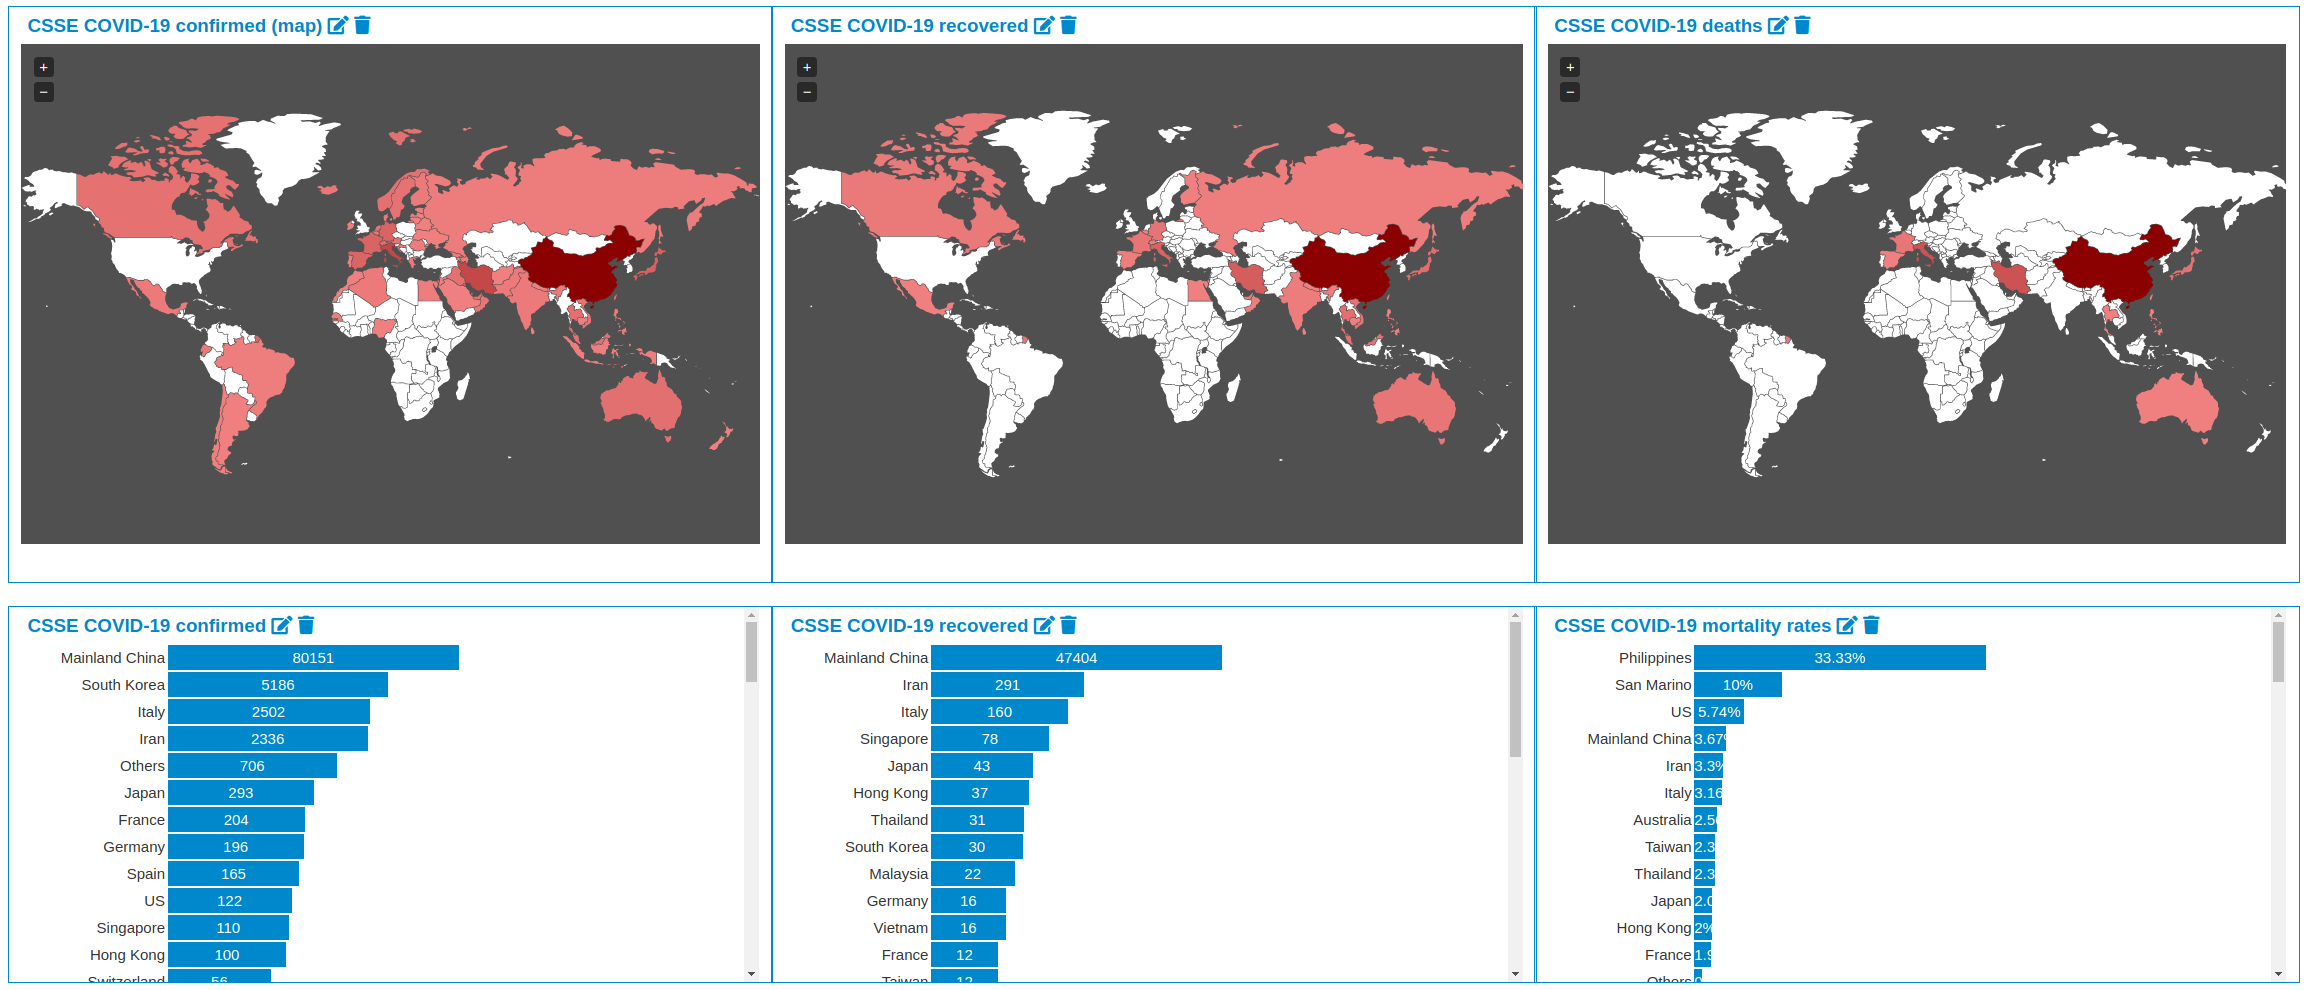
\includegraphics[scale=0.18]{dashboard_small.png}
  \end{center}
\end{frame}

\begin{frame}
  \frametitle{The internals of awidget}
        \begin{itemize} 
            \item {\bf Backend} for the widget, full access to all MISP internals
            \item {\bf Load, convert, format} to be represented via view widgets
            \item {\bf Widget metadata} - size, name, description, behaviours
            \item Only main function required to be implemented: {\bf handler()}
            \item Optional: {\bf checkPermissions() for ACL}
            \item Accepts {\bf user configuration} for which a template can be provided
            \item Located in /var/www/MISP/app/Lib/Dashboard/
            \item Custom widgets can be placed in /var/www/MISP/app/Lib/Dashboard/Custom/
        \end{itemize}
\end{frame}

\begin{frame}
  \frametitle{The view layer of a widget}
  \begin{itemize}
        \item View files are included by default and reusable
        \item Currently we have a small but growing list of views
        \begin{itemize}
            \item BarChart
            \item SimpleList
            \item WorldMap
        \end{itemize}
        \item Converts the data passed by the Widget logic to HTML
        \item Located in /var/www/MISP/view/Elements/dashboard/Widgets/
  \end{itemize}
\end{frame}

\begin{frame}
  \frametitle{Widget behaviours}
  \begin{itemize}
    \item Widgets can additionally be tied to certain {\bf behaviours}:
    \begin{itemize}
      \item Caching
      \begin{itemize}
        \item Executions of the widget logic are cached
        \item {\bf Separate caches for each organisation in addition to site admins}
        \item Cache duration is controlled by the widget logic
      \end{itemize}
      \item Refresh
      \begin{itemize}
        \item Widgets can be set to refresh after x seconds
      \end{itemize}
      \item Both of these should be used with special care in regards to the use of {\bf system resources}
    \end{itemize}
  \end{itemize}
\end{frame}

\begin{frame}
    \frametitle{Exercise module: simple Whoami}
    \begin{itemize}
        \item Let's start with a skeleton
        \item Create /var/www/MISP/app/Lib/Dashboard/Custom/WhoamiWidget.php
        \item MISP will parse anything ending with Widget.php in this directory
    \end{itemize}
\end{frame}

\begin{frame}[fragile]
    \frametitle{Exercise module: simple Whoami}
    \begin{adjustbox}{width=\textwidth,height=8cm,keepaspectratio}
        \begin{lstlisting}[language=json,firstnumber=1]
<?php
class MispWhoamiWidget
{
  public $title = 'Whoami';
  public $render = 'SimpleList';
  public $width = 2;
  public $height = 2;
  public $params = array();
  public $description = 'Shows information about the currently logged in user.';
  public $cacheLifetime = false;
  public $autoRefreshDelay = 3;

  public function handler($user, $options = array())
  {
    $data = array();
    return $data;
  }
}
        \end{lstlisting}
    \end{adjustbox}
\end{frame}

\begin{frame}
  \frametitle{Meta information}
  \begin{itemize}
    \item {\bf \$title}: The name of the widget
    \item {\bf \$description}: A description of the widget
    \item {\bf \$render}: The view element to use in rendering the widget
    \item {\bf \$width \& \$height}: Default relative dimensions
    \item {\bf \$params}: Configuration array with explanations for each key
    \item {\bf \$cacheLifetime}: The lifetime of the caches in seconds (false disables it)
    \item {\bf \$autoRefreshDelay}: The time in seconds between each refresh (false disables it)
  \end{itemize}
  
\end{frame}

\begin{frame}[fragile]
  \frametitle{The handler}
    \begin{adjustbox}{height=4cm,keepaspectratio}
        \begin{lstlisting}[language=json,firstnumber=1]
public function handler($user, $options = array())
{
  $this->Log = ClassRegistry::init('Log');
  $entries = $this->Log->find('all', array(
    'recursive' => -1,
    'conditions' => array(
      'action' => 'login', 'user_id' => $user['id']
    ),
    'order' => 'id desc',
    'limit' => 5,
    'fields' => array('created', 'ip')
  ));
  foreach ($entries as &$entry) {
    $entry = $entry['Log']['created'] . ' --- ' .
    (
      empty($entry['Log']['ip']) ?
      'IP not logged' :
       $entry['Log']['ip']
    );
  }
  return array(
    array('title' => 'Email', 'value' => $user['email']),
    array(
      'title' => 'Role', 'value' => $user['Role']['name']
    ),
    array(
      'title' => 'Organisation',
      'value' => $user['Organisation']['name']
    ),
    array(
      'title' => 'IP', 'value' => $_SERVER['REMOTE_ADDR']
    ),
    array('title' => 'Last logins', 'value' => $entries)
  );
}
        \end{lstlisting}
    \end{adjustbox}
\end{frame}

\begin{frame}
  \frametitle{Result}
  \begin{center}
    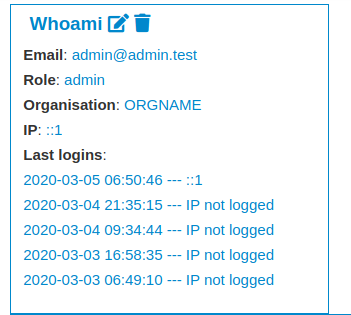
\includegraphics[scale=0.5]{whoami.png}
  \end{center}
\end{frame}

